% arara: pdflatex: { synctex: yes }
% arara: makeindex: { style: ctuthesis }
% arara: bibtex

% The class takes all the key=value arguments that \ctusetup does,
% and a couple more: draft and oneside
\documentclass[oneside]{ctuthesis}

\ctusetup{
%	preprint = \ctuverlog,
	mainlanguage = english,
	otherlanguages = {czech},
	title-english = {NLP Methods for Automated Fact-Checking},
	xdoctype = M,
	xfaculty = F3,
	department-english = {Department of Computer Science},
	author = {Ing. Herbert Ullrich},
	supervisor = {Ing. Jan Drchal, Ph.D.},
	fieldofstudy-english = {Informatics},
	subfieldofstudy-english = {Natural Language Processing},
	keywords-czech = {Fact-checking, Natural Language Inference, Claim Generation, Transformers, LLMs},
	keywords-english = {Fact-checking, Natural Language Inference, Claim Generation, Transformers, LLMs},
	day = 21,
	month = 8,
	year = 2023,
	pkg-listings = true
%	monochrome = true,
%	layout-short = true,
}

\ctuprocess

\ctutemplateset{maketitle twocolumn default}{
	\begin{twocolumnfrontmatterpage}
		%\ctutemplate{twocolumn.thanks}
		%\ctutemplate{twocolumn.declaration}
		%\ctutemplate{twocolumn.abstract.in.titlelanguage}
		%\ctutemplate{twocolumn.abstract.in.secondlanguage}
		\ctutemplate{twocolumn.tableofcontents}
		\ctutemplate{twocolumn.listoffigures}
	\end{twocolumnfrontmatterpage}
}

% Theorem declarations, this is the reasonable default, anybody can do what they wish.
% If you prefer theorems in italics rather than slanted, use \theoremstyle{plainit}
\theoremstyle{plain}
\newtheorem{theorem}{Theorem}[chapter]
\newtheorem{corollary}[theorem]{Corollary}
\newtheorem{lemma}[theorem]{Lemma}
\newtheorem{proposition}[theorem]{Proposition}

\theoremstyle{definition}
\newtheorem{definition}[theorem]{Definition}
\newtheorem{example}[theorem]{Example}
\newtheorem{conjecture}[theorem]{Conjecture}

\theoremstyle{note}
\newtheorem*{remark*}{Remark}
\newtheorem{remark}[theorem]{Remark}

\DeclareMathOperator*{\argmin}{arg\!min}
\DeclareMathOperator*{\argmax}{arg\!max}


% Only for testing purposes
\listfiles
\usepackage[pagewise]{lineno}
\usepackage{lipsum,blindtext}
\usepackage{mathrsfs} % provides \mathscr used in the ridiculous examples

% TODO: filter out unnecessary pckgs
%\usepackage[breaklinks=true]{hyperref}
%\usepackage{breakcites}
\usepackage{cite}
%\usepackage{mathtools}
%\usepackage{amsmath}
%\usepackage{amsfonts}
%\usepackage{amssymb}
%\usepackage{algpseudocode}
%\usepackage{algorithm}
\usepackage{xcolor}
\usepackage{xspace}
\usepackage[ruled,lined,linesnumbered, commentsnumbered]{algorithm2e}
%\usepackage{listings}
%\usepackage{caption}
\usepackage{subcaption}
\usepackage{enumerate}
\usepackage{tabularx}
%\usepackage{hyperref}
\usepackage{tablefootnote}
\usepackage{hhline}
\usepackage{multirow}
\usepackage{dcolumn}

\def\"#1{``#1''}
\def\btn#1{{\itembox{\textbf{\textsf{#1}}}}}
\def\db#1{{{\textit{\textsf{#1}}}}}
\def\todo#1{{\textcolor{red}{{\techbf TODO:} {#1}}}}
\def\tnula{\hyperref[t0]{$\textsf{T}_{\textsf{0}}$}}
\def\tjednaa{\hyperref[t1a]{$\textsf{T}_{\textsf{1a}}$}}
\def\tjednab{\hyperref[t1b]{$\textsf{T}_{\textsf{1b}}$}}
\def\tdvaa{\hyperref[t2a]{$\textsf{T}_{\textsf{2a}}$}}
\def\tdvab{\hyperref[t2b]{$\textsf{T}_{\textsf{2b}}$}}
\def\tdva{\hyperref[t2a]{$\textsf{T}_{\textsf{2}}$}}

\newcommand{\train}{\textsf{train}\xspace}
\newcommand{\dev}{\textsf{dev}\xspace}
\newcommand{\test}{\textsf{test}\xspace}

\newcommand{\SUP}{\texttt{SUPPORTS}}
\newcommand{\REF}{\texttt{REFUTES}}
\newcommand{\NEI}{\texttt{NEI}}

\newcommand{\FEVER}{\textsc{FEVER}\xspace}
\newcommand{\FEVERNLI}{\textsc{FEVER-NLI}\xspace}
\newcommand{\Wikipedia}{\textsc{Wikipedia}\xspace}
\newcommand{\MediaWiki}{\textsc{MediaWiki}\xspace}
\newcommand{\FCZ}{\textsc{CsFEVER}\xspace}
\newcommand{\FCZNLI}{\textsc{CsFEVER-NLI}\xspace}
\newcommand{\FEN}{\textsc{EnFEVER}\xspace}
\newcommand{\FDAN}{\textsc{DanFEVER}\xspace}
\newcommand{\CTK}{\textsc{CTKFacts}\xspace}
\newcommand{\CTKNLI}{\textsc{CTKFactsNLI}\xspace}
\newcommand{\Anserini}{\textsc{Anserini}\xspace}
\newcommand{\DrQA}{\textsc{DrQA}\xspace}
\newcommand{\BERT}{\textsc{Bert}\xspace}
\newcommand{\RoBERTa}{\textsc{RoBERTa}\xspace}
\newcommand{\MBERT}{\textsc{M-Bert}\xspace}
\newcommand{\SMBERT}{\textsc{Sentence M-Bert}\xspace}
\newcommand{\ColBERT}{\textsc{ColBert}\xspace}
\newcommand{\SlavicBERT}{\textsc{SlavicBERT}\xspace}
\newcommand{\CZERT}{\textsc{Czert}\xspace}
\newcommand{\RobeCzech}{\textsc{RobeCzech}\xspace}
\newcommand{\XLM}{\textsc{XLM-RoBERTa}\xspace}
\newcommand{\FERNETC}{\textsc{FERNET-C5}\xspace}
\newcommand{\FERNETN}{\textsc{FERNET-News}\xspace}
\newcommand{\XLMSQUAD}{\textsc{XLM-RoBERTa @ SQuAD2}\xspace}
\newcommand{\XLMXNLI}{\textsc{XLM-RoBERTa @ XNLI}\xspace}


\begin{document}

\maketitle

%!TEX ROOT=../ctutest.tex

\chapter{Introduction}
\label{chap:intro}

Our dissertation, as well as our long-term research, centers around the field of \textit{automated fact checking} through the means of Natural Language Processing and its modern methods.
The work consists of the analysis of the whole fact-checking process, its subdivision and simplification into tasks that can be efficiently addressed using the current state-of-the-art NLP methods, collection of data appropriate to benchmark such tasks, delivery of example solutions and their validation against similar research in other languages and related tasks.

Our main focus are the fact-checking-related tasks in the West Slavic languages (Czech, Slovak and Polish) and secondarily in English.
Our contribution has so far been the collection and publication of novel datasets for the fact-checking task and its subroutines, models trained for the tasks and their debate, including the ongoing establishment of metrics that would rate the model success and error rates in terms close to the human notion of \textit{facticity} (which proves to be a challenge on its own, requiring another round of novel research). 

Our doctoral aim is to cover every step on the path from gathering a factual claim -- for example, extracting it from a political debate -- to predicting its veracity verdict and justifying it rigorously with hard data.
With the recent boom in NLP beginning with the advent of transformer networks and later the Large Language Models, prompting and few-shot learning, a significant part of the research is and has to be an appropriate and timely adoption of new ever-evolving sota NLP solutions, based on well-designed studies in our specific context.

Overall, our agenda is to follow up on our published research on fact checking in Czech with methods that reiterate on our results in other languages and evolving our previous methodology based on transformer \textit{pre-training \& fine-tuning} paradigm to a computationally feasible design based on LLMs. 
We want to establish the task of \textit{claim generation} among the other commonly benchmarked NLP tasks within the scientific community, adjacent to that of \textit{abstractive summarization}.
We aim to give safeguards and explanations to the model decisions with human-understandable metrics, in particular revealing hallucinations -- a common problem of modern day LLMs.

The goal of this study is to show the directions we are taking to address these challenges, reasoning behind them, our research questions and current results that motivated them.

\section{Motivation}
\label{sec:motivation}

The spread of misinformation in the online space has a growing influence on the Czech public~\cite{stem}. It has been shown to influence people's behaviour on the social networks~\cite{Lazer1094} as well as their decisions in elections~\cite{10.1257/jep.31.2.211}, and real-world reasoning, which has shown increasingly harmful during the COVID-19 pandemic~\cite{BARUA2020100119}.

The recent advances in artificial intelligence and its related fields, in particular the recommendation algorithms, have contributed to the spread of misinformation on social media~\cite{doi:10.1177/2056305119888654}, as well as they hold a large potential for automation of the false content generation and extraction of sensational attention-drawing headlines -- the \"{clickbait} generation~\cite{shukai}.

Recent research has shown promising results~\cite{fever2} in false claim detection for data in English, using a trusted knowledge base of true claims (for research purposes typically fixed to the corpus of \textsf{Wikipedia} articles), mimicking the \textit{fact-checking} efforts in journalism.

Fact-checking is a rigorous process of matching every information within a \textit{factic claim} to its \textit{evidence} (or \textit{disproof}) in trusted data sources to infer the claim veracity and verifiability. In exchange, if the trusted \textit{knowledge base} contains a set of \"{ground truths} sufficient to fully infer the original claim or its negation, the claim is labelled as {\techbf{supported}} or {\techbf{refuted}}, respectively. If no such \textit{evidence set} can be found, the claim is marked as {\techbf{unverifiable}}\footnote{Hereinafter labelled as \texttt{NOT ENOUGH INFO}, in accordance to related research.}.


\section{Challenges}

\begin{figure}
    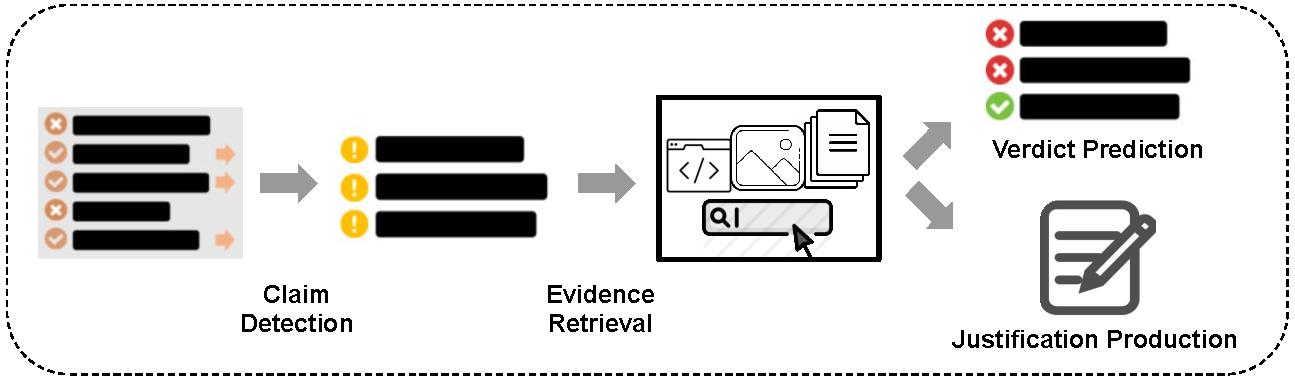
\includegraphics[width=14cm]{fig/framework.pdf}
    \caption{Automated fact-checking pipeline, reprinted from~\cite{guo-etal-2022-survey}}
    \label{fig:framework}
\end{figure}

Despite the existence of end-to-end fact-checking services, such as \url{politifact.org} or \url{demagog.cz}, the human-powered approach shows weaknesses in its scalability. By design, the process of finding an exhaustive set of evidence that decides the claim veracity is much slower than that of generating false or misguiding claims. Therefore, efforts have been made to move part of the load to a computer program that can run without supervision.

The common research goal is a fact verification tool that would, given a claim, semantically search provided knowledge base (stored for example as a \textit{corpus} of some natural language), propose a set of evidence (e. g. $k$ semantically nearest paragraphs of the corpus) and suggest the final verdict (Figure \ref{fig:pipeline}). This would reduce the fact-checker's workload to mere adjustments of the proposed result and correction of mistakes on the computer side. 

The goal of the ongoing efforts of {\textsf{FactCheck}} team at {\textsf{AIC CTU}}, as addressed in the works of~\cite{rypar,dedkova} and~\cite{gazo} is to explore the state-of-the-art methods used for fact verification in other languages, and propose a strong baseline system for such a task in Czech.


\section{A word on the Transformers}
\label{sec:transformers}
For the past six years, the state-of-the-art solution for nearly every Natural Language Processing task is based on the concept of \textit{transformer networks} or, simply, \textit{Transformers}. This has been a major breakthrough in the field by~\cite{vaswani}, giving birth to the famous models such as \textsf{Google}'s \textsf{BERT}~\cite{bert} and its descendants, or the \textsf{OpenAI}'s \textsf{GPT-3}~\cite{gpt3}.

In our proposed methods, we use Transformers in every step of the fact verification pipeline. Therefore, we would like to introduce this concept to our reader to begin with. 

Transformer is a neural model for \textit{sequence-to-sequence} tasks, which, similarly e.g. to the \textit{LSTM-Networks}~\cite{lstm}, uses the Encoder--Decoder architecture. Its main point is that of using solely the \textit{self-attention} mechanism to represent its input and output, instead of any sequence-aligned recurrence~\cite{vaswani}.

In essence, the \textit{self-attention} (also known as the \textit{intra-attention}) transforms every input vector to a weighted sum of the vectors in its neighbourhood, weighted by their \textit{relatedness} to the input. One could illustrate this on the \textit{euphony} in music, where every tone of a song relates to all of the precedent ones, to some more than to the others.

The full Transformer architecture is depicted in Figure~\ref{fig:transformer}.
%--- FIG: UTF forms
\begin{figure}
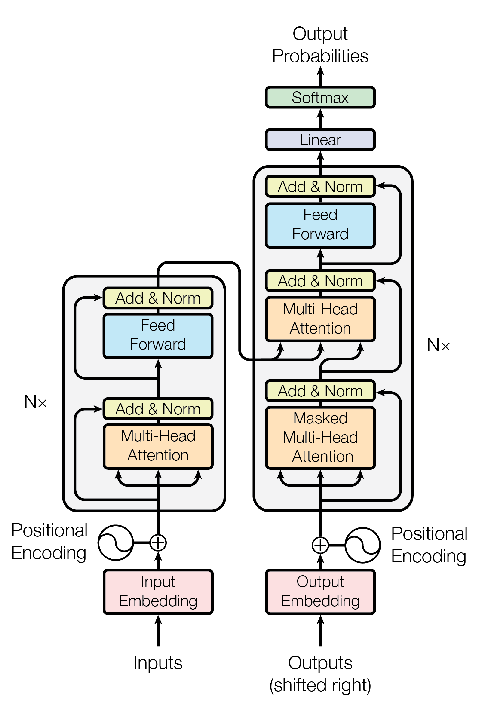
\includegraphics[width=9cm]{fig/transformer.pdf}
\caption{Transformer model architecture, reprinted from~\cite{vaswani}}
\label{fig:transformer}
\end{figure}
%--- /FIG



\section{Dissertation minimum study outline}
 
\begin{itemize}
\item {\techbf{Chapter~\ref{chap:intro}}} introduces the dissertation topic, motivates the research sets up our challenges for the future research 

\item {\techbf{Chapter~\ref{chap:sota}}} examines the most relevant research in the field and tries to highlight the recent paradigm shift from models trained for a single task to a single large models that perform well in everything

\item {\techbf{Chapter~\ref{chap:contribution}}} explains our current contributions to the field of automated fact-checking and NLP in Chech

\item {\techbf{Chapter~\ref{chap:plan}}} describes our plan for the dissertation and justifies the directions we are taking

\item Finally, {\techbf{Chapter~\ref{chap:conclusion}}} concludes the study with a wrapup of its findings

\end{itemize}


%!TEX ROOT=../ctutest.tex

\chapter{State of the Art}
%--- FIG: UTF forms

This chapter will first describe the originally popular models for general NLP, such as BERT and the recent paradigm shift from \textit{pretrain + finetune} transfer learning framework popular since the original~\cite{devlin2019bert} paper to the currently booming LLMs, which often outperform the smaller models even without the fine-tuning step~\cite{gpt4, llama, vicuna}. We will then take a look at the performance optimization methods that enable training multi-billion parameter pre-trained models on a set of task-specific data on a single GPU and their potential for our research. 

To show how it relates to our main topics, we will introduce currently published approaches for the automated fact-checking task, efforts related to claim generation, and evaluation of NLP model outputs.

\label{chap:sota}
\section{Pretrain + Finetune}
\label{sec:pretrain}
For the last decade, the \textit{pretrain-finetune} paradigm has been a cornerstone in Natural Language Processing (NLP). It has significantly shaped the development of modern NLP models. Its use in NLP can be traced back to the advent of neural networks and deep learning in the early 2010s. Initially, researchers pre-trained word embeddings using methods like Word2Vec~\cite{mikolov} and GloVe~\cite{pennington-etal-2014-glove}, which captured semantic relationships among words and then tweaked the general-task models for various related tasks.

\subsection{BERT and derivatives}\label{sec:bert}
The \textit{pretrain-finetune} paradigm truly rose to fame with the introduction of transformer-based models, particularly the revolutionary BERT (Bidirectional Encoder Representations from Transformers) in 2018. BERT~\cite{devlin2019bert} demonstrated the power of pretraining large-scale language models on massive text corpora using an easy-to-automate general task such as \textit{Masked Language Modeling}, or \textit{Next Sentence Prediction}, followed by fine-tuning on specific downstream tasks using smaller, harder-to-obtain data. This approach achieved state-of-the-art results across various NLP benchmarks. Subsequently, numerous variations of pre-trained models like GPT (Generative Pre-trained Transformer) and RoBERTa emerged, each refining the pretrain-finetune paradigm to improve language understanding, generation, and transfer learning capabilities. 

Importantly, BERT's success inspired many publications in training similar transformer models, varying in the definition of the general pre-training task, model size, architecture training corpus

\begin{itemize}
    \item In Czech language, monolingual models CZERT~\cite{czert}, FERNET~\cite{fernet}, RobeCzech~\cite{straka2021robeczech}, and small-e-czech~\cite{kocian2021siamese} are available for further finetuning
    \item In Polish, HerBERT~\cite{mroczkowski-etal-2021-herbert} achieved state-of-the-art in multiple tasks in 2021
    \item In Slovak, SlovakBERT~\cite{pikuliak2021slovakbert} was released by KInIT and Gerulata
    \item A multitude of multilingual models, such as \MBERT or \XLM~\cite{xlm-roberta} were pre-trained on data in all three of these languages (and many others), proving that the large transformers can capture a notion of semantics and relations between pieces of text even \textit{without} the convenient constriction of a single language 
\end{itemize}

\section{Few-shot and Zero-shot learning}
\label{sec:llms}
The ever-growing (sometimes billions of parameters in size) transformer models have not only demonstrated superior performance on benchmark datasets but have also shown remarkable zero-shot and few-shot learning abilities, where they can perform tasks with minimal or no task-specific training data~\cite{gpt3}.

Few-shot learning refers to the capability of a model to perform a task when provided with only a limited amount of labeled examples. Zero-shot learning takes this concept a step further by enabling models to tackle tasks they have never seen during training. The integration of these learning paradigms into large language models like GPT-3 and subsequent iterations has spread the NLP hype even further. By utilizing a prompt or a few examples, these models can quickly adapt to new tasks, making them highly versatile, adaptable, and usable to the general public.
\subsection{OpenAI LLMs: GPT-3 and GPT-4}
\label{sec:gpt}
In 2020, the few-shot learning was exhibited on GPT3 -- a 175B-parameter autoregressive model trained by~\cite{gpt3}. The model was trained on the task of generating text based on user's and its own previous outputs.
The training procedure and data\footnote{A mixture of crawled websites, books, and Wikipedia.} is thoroughly described in the publication. However, it is prohibitively costly for most labs to reproduce or even fine-tune at such a scale. 

In the fall of 2022, GPT-3 became widely popular thanks to its \textsf{ChatGPT}\footnote{\url{https://chat.openai.com}} fine-tune and demonstration app, which puts the user in the role of \textit{prompter}, texting back and forth with an LLM that predicts the most fitting reply to each conversation.

With the arrival of GPT-4, the \textsf{ChatGPT} was already massively famous, and the new model already shipped with a paid-service business scheme no longer publishing the training data, tasks, or even model size~\cite{gpt4}.

\section{Open source LLMs}
This puts the research community in an awkward position, as the GPT-4 achieves state-of-the-art in numerous NLP benchmarks~\cite{gpt4, Liu_2023}, but is designed not to be used in any way other than as a black box, making the derived research rigorosity and reproducibility disputable.

From the prediction times, \textsf{OpenAI} claims, and general trends in NLP, there are also reasons to believe that GPT-4 is orders of magnitude larger than already wasteful GPT-3.
This motivates an uptick in research of other LLMs that would be able to operate on a smaller scale with similar results, using a peer-reviewed architecture, training scheme, and data that is available in open source.

\subsection{LLaMA-2 and derivatives}
\label{sec:llama}

A popular foundational LLM to compete with the GPT family has become the \textsf{LLaMA}~\cite{llama} from \textsf{Meta research}. LLaMA was trained on about 5TB of publicly available textual data\footnote{To be specific, LLaMA was trained using an autoregressive language modeling task on a mixture of English CommonCrawl Corpus, C4~\cite{raffel2020exploring}, Github, Wikipedia, Gutenberg Project, Books3 corpus, ArXiv and Stack Exchange} mainly in English. 

It comes in various sizes between 7B and 65B parameters, achieving a SOTA among open-source solvers in various tasks and an unmatched performance in the field of single-GPU (7B and 13B) model sizes.
LLaMA proceeds to be used as a goto base model for a number of successful open-source chatbots such as Alpaca~\cite{alpaca}, Vicuna~\cite{vicuna}, and OpenAssistant~\cite{openassistant}.

The pre-trained LLaMA weights are, however, published under a restrictive license that prohibits republishing the model weights even after tuning its parameters, which limits its fine-tuners to publishing delta- or xor-weights that can not be properly used without \textsf{Meta}'s permission.

LLaMA-2~\cite{llama2} addresses this inconvenience (as well as delivers its own take on the \textit{chatbot} task), yielding an ideal strong base model for experimentation with any NLP task in 7B, 13B, and 70B sizes.
The only obstacle left in the way is the computational cost of fine-tuning across so many parameters.

%Open-source, freely usable.
%Often poor czech coverage 
%Quantizace, 4b, 8b, zlomek parametrů\cite{openassistant}

\subsection{LoRA and other optimization}\label{sec:lora}
To be able to fine-tune multi-billion-parameter models such as \textsf{LLaMA-2}~\cite{llama2} on a single TPU, successful approaches have been published to dramatically cut down the training expenses.
Parameter-efficient fine-tuning (PEFT)~\cite{peft} proposes approaches to only fine-tune \textit{a few} weights as opposed to the whole neural network, reducing the number of trainable parameters by orders of magnitude.
Low-Rank Adaptation of Large Language Models (LoRA)~\cite{lora} does so by freezing the pre-trained model weights and injecting trainable rank decomposition matrices into each layer of Transformer architecture. 

Quantization, which cuts the costs of working with 32- or 16-bit float parameters and opting for data types of bitsize as small as 4, also proves to be a powerful tool for LLM finetuning performance optimization~\cite{dettmers2023qlora}.
Quantized QLoRA takes LLaMA and finetunes it into a Guanaco model family, which outperforms all previous openly released LLMs on Vicuna benchmark~\cite{dettmers2023qlora} and achieves 99.3\% of the ChatGPT's performance on it while only requiring 24 hours on a single GPU.

As per an alleged leaked Google memo~\cite{moat}, this could put the future state of the art in NLP disciplines back into the hands of open source and public research, not giving any of the big tech companies a \"{moat} advantage.

Either way, it goes to show that the open-source LLMs have a promising future in NLP and will be indismissible as an approach for the NLP task of \textit{Automated fact checking}.

\section{Fact checking approaches}
Back in the late 2010s, the misinformation and its spread in the era of the internet and social media became a discussed topic in the Western world, with multiple institutions such as the European Council marking it a severe threat to democracy and national safety~\cite{disorder}.
The public attention and maturation of appropriate technologies motivated numerous efforts in business and academia to tackle the challenge.
Among other events, a Fake News Challenge occurred in 2017~\cite{fncweb} exploring the uses of technologies in the field and applying, for example, the LSTMs to detect stances among textual data~\cite{fnc}.

\subsection{FEVER and followups}
Soon, standard tasks began to be formulated and data collected. 
The FEVER (Fact Extraction and VERification)~\cite{fever} dataset and shared task became prominent in natural language processing research.
Relatively early on, it formalized the task as a two-step problem:
\begin{enumerate}
    \item Retrieving information within a structured corpus to fact-check a given claim (this resembles a standard NLP problem called \textit{information retrieval} -- IR)
    \item Classifying the inference relation between retrieved information and claim as one of:
    \begin{enumerate}
        \item {\techbf supports} -- information semantically implies the claim 
        \item {\techbf refutes} -- information semantically implies the negation of the claim 
        \item {\techbf not enough info} otherwise 
    \end{enumerate}
    This classification task became known as \textit{natural language inference} and mostly replaced the previous binary classification NLP task of \textit{recognizing textual entailment} (RTE)
\end{enumerate}

The FEVER dataset was a collection of 185K human-annotated claims, their veracity labels, and sets of evidence from a structured corpus that sufficed to justify the labels.
The corpus of choice was a 2017 English Wikipedia structured into articles due to its reasonable size, informational richness, and open license.\footnote{Is Wikipedia a trustworthy informational canon, though? 
No, it is not supposed to -- FEVER states that it is crucial to always maintain that the fact-checking classifiers only classify \textit{with respect to} data, and their reliability goes only as far as that of the underlying knowledge corpus. Therefore, \textit{supports} does not directly translate to \textit{true}, nor \textit{refutes} to \textit{false}}

FEVER yields an interesting benchmark with statistically quantifiable model success, motivated multiple well-performing public solutions~\cite{fever1,fever2}, gives insights into the complexities of automated fact-checking task, and strong baselines for research in the field. The data was later enriched by contrastive evidence in VitaminC~\cite{DBLP:journals/corr/abs-2103-08541} and by reasoning over tabular data in FEVEROUS~\cite{aly2021feverous}.

To date, it keeps being a reference point in automated fact-checking research despite its limitations, such as its requirement for a fixed knowledge base and \"{atomicity}\footnote{See section 4.1.2.\ref{atomicity}} of claims.

\begin{figure}
    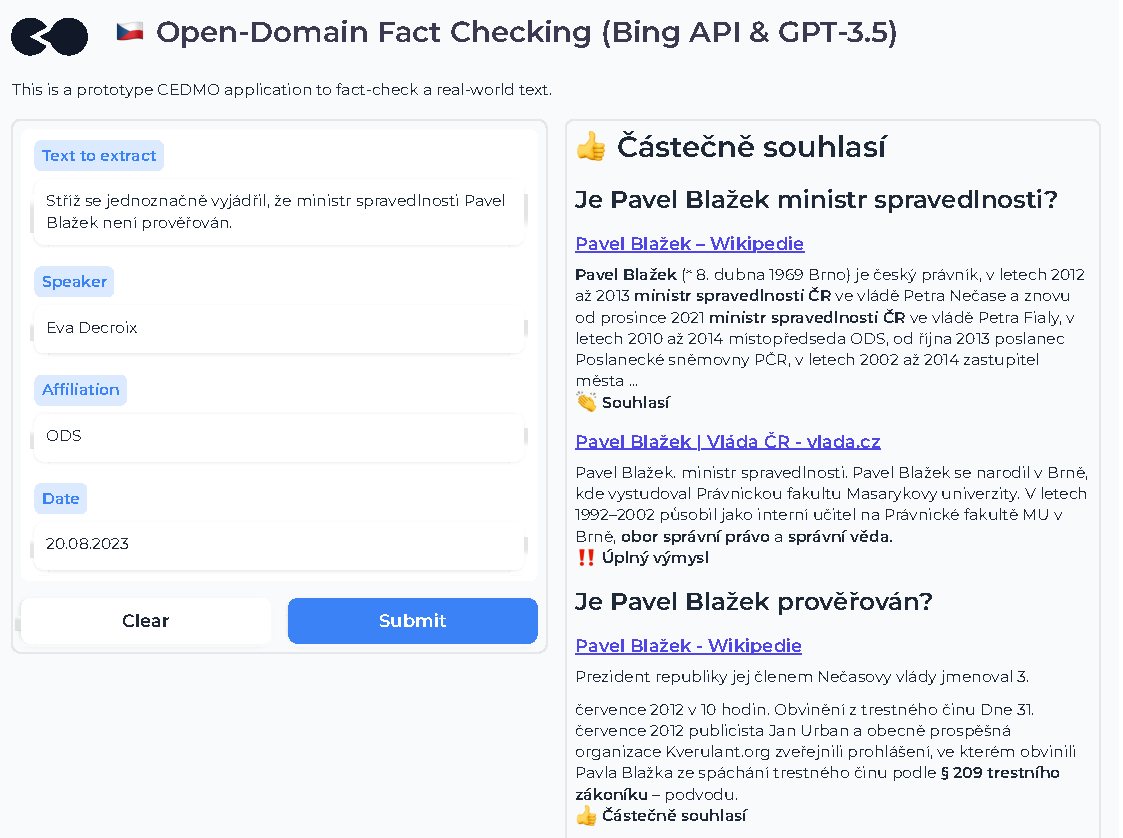
\includegraphics[width=14cm]{fig/bing.pdf}
    \caption{Proof-of-concept Czech fact-checking based on live-internet search (Bing API) and LLM prompting, based on the proposals of~\cite{bing} in Czech, using a real-world claim that was fact-checked by \href{https://demagog.cz/vyrok/22849}{\url{demagog.cz}} in June 2023}
    \label{fig:bing}
\end{figure}

\subsection{Open-domain fact-checking}
Due to these limitations, some researchers consider the scheme from FEVER an oversimplification -- the real politics' claims to be fact-checked by journalists often consist of long syntactical structures, combine information together in a non-trivial manner and often require the most up-to-date evidence. 

\"{Complex Claim Verification with Evidence Retrieved in the Wild}~\cite{bing} proposes a different scheme that overcomes these shortcomings:

\begin{enumerate}
    \item Arbitrarily complex claim is decomposed into a set of yes/no questions
    \item An open-domain search (Bing is proposed in the paper) fetches several evidence documents for each question
    \item A claim-focused summary is extracted from each document
    \item A veracity classifier goes through each pair of evidence and question, ranging from \"{faithful} to \"{completely wrong}
    \item The scores are combined (all need to be \"{faithful} for a faithful claim. Otherwise, the severity of inaccuracies can be approximated using some averaging.
\end{enumerate}

GPT-3 is used in steps 1, 3, and 4 of the scheme in the prototype delivered in~\cite{bing} in a few- and zero-shot fashion, with few-shot unsurprisingly coming out a little better. The scheme is transducible to Czech, and Figure~\ref{fig:bing} shows my early experiments with my interactive reproduction of it, predictors based on Bing and GPT-3.5 (a polished version of GPT-3).

While the shift from an established FEVER framework to complex real-world claims and evidence retrieval \"{in the wild} feels exciting and practical, an obvious pitfall arises -- anyone can publish anything on the internet, having it appear in Bing search and other crawlers alike. I argue that this might lead into a sort of a circular dependency of needing to reliably fact-check the evidence we have retrieved from the web in order to be able to build a reliable fact-checker in the first place.

Anyhow, the open-domain fact-checking idea opens a whole new range of approaches and shows the power of LLMs in fact-checking at its every step.

\section{Claim generation}
Another step of the fact-checking pipeline, covered by very few research publications, is the generation of the claim to be checked in the first place~\cite{guo-etal-2022-survey}.

The current state of things is that journalists who fact-check statements within, say, a Facebook status, need to read through the whole document multiple times, formulate its factual claims from the stances and facts expressed in the text themselves, and then fact-check each separately.

What has been examined so far were, for example:
\begin{itemize}
    \item Using Question Generation (QG) solver and converting the questions into declarative sentences to emulate more claims and more data for fact checking~\cite{pan2021zeroshot}
    \item Numerous CLEF CheckThat! challenges explored the task of estimating \textit{checkworthiness} of different parts of a long text, such as lines in a political debate~\cite{clef19,clef21}
    \item The task of extreme summarization (XSum) consists of summarizing a long body of text into a single sentence, focusing on its most relevant aspects and facts. Large datasets XSum~\cite{narayan-etal-2018-dont} in English and XL-Sum~\cite{xlsum} in 44 languages both present expertly annotated data from BBC News for it, as their article standard features a single-sentence summary at the beginning of each text.
\end{itemize}

\subsection{NLP summarization benchmarking}
\label{benchmarking-sota}
An important caveat to note with the NLP tasks reducing longer text to shorter text -- such as summarization or claim extraction -- is that the standard automatic metrics such as ROUGE~\cite{lin-2004-rouge} and METEOR~\cite{banerjee-lavie-2005-meteor} only focus on the \textit{content selection} aspect of tasks, based on a word-by-word overlap and were designed to use on multiple gold summaries per input, which are not often provided with modern large-scale datasets.~\cite{nlpprogress,bert-score,zha2023alignscore}

These serious limitations make it questionable for anyone to claim state-of-the-art on these tasks and motivate research for new metrics to cover all the important aspects of claim generation and do so in correlation with expert human judgment. 

This will be the topic of section~\ref{metrics}, which also introduces the state-of-the-art research we are working with to arrive to a valid set of benchmarks.
%!TEX ROOT=../ctutest.tex

\chapter{Current Contribution}
\label{chap:contribution}

\textit{We have collected novel data for the fact-checking task in our application context, emulated and scraped inavailable datasets making them public or readying them for doing so, we have established numerous state-of-the-art models and we are currently working on establishing the topic of claim generation as a summarization-related NLP task.}

\section{Datasets}
Having the automated fact-checking scheme established in chapter~\ref{chap:sota}, every machine-learning solution must start with the choice or collection of appropriate training data.
Due to the novelty of the task in Czech and other West Slavic languages, I explored a multitude of ways to acquire such data, many of them resulting in a publicly available dataset in our Huggingface repository~\footnote{\url{https://huggingface.co/ctu-aic}}, beginning to be reused by others. 

\subsection{\FCZ}\label{sec:fcz}
An early \"{temporary benchmark} for our endeavours in adapting the FEVER~\cite{fever} task for the Czech context was the \FCZ~\cite{lrev} dataset.

In~\cite{diplomka}, I have proposed a simple FEVER data transduction scheme that can be simplified as follows:

\begin{enumerate}
    \item Each FEVER claim is translated using the (at the time maturing) Machine Translator
    \item Evidence from English Wikipedia is not translated using MT, but mapped onto its Czech-Wikipedia counterpart using the publicly available Wikidata\footnote{Used, for example, for showing the \"{see this article in other languages} suggestions in Wikipedia sidebar}
    \item Data with any loss in evidence due to the step 2. is discarded
\end{enumerate}

This design was relatively cheap to compute (as translating the whole 2017 Wikipedia corpus would have been a long and wasteful computation), delivering an open-license dataset of 127K claims, their labels and evidence justifications. My hope was, as both the 2017 EnWiki and our 2020 CsWiki corpus only featured the first paragraph (abstract) of each article, a document-level alignment could be assumed -- both the Czech and English text always summarize the basic facts about the same entity.

This showed to be only partly true as a later human annotation on a 1\% sample of \FCZ data showed that about a third of data exhibits some levels of noise, mostly introduced during dataset translation~\cite{lrev}.

While noisy, the \FCZ data still got its use in training of the information retrieval schemes of~\cite{rypar,gazo,lrev} used to this day and is openly available\footnote{\url{https://huggingface.co/datasets/ctu-aic/csfever}} under a CC license.

My research on it also motivated a creation of a inference-only version of the dataset, which does not support the Information Retrieval task and therefore, does not require the mapping of evidence into a live version of Wikipedia.
Therefore, only the EnWiki \textit{excerpts} needed to build evidence can be translated, bringing down the computational difficulty and enabling me to deliver a dataset without the transduction noise called \FCZNLI\footnote{\url{https://huggingface.co/datasets/ctu-aic/csfever_nli}}. 

Another round of research \FCZ motivated and I supervised was the successful thesis of~\cite{mlynar}, modernizing the data and machine-translation methods into the 2023 state of the art.
\cite{mlynar} further experimented with methods of automated noise detection and removal, which has not shown to be an efficient way to tackle the issue of high noise in \FCZ.

However, it delivers a partly cleaned versions of it\footnote{\url{https://huggingface.co/datasets/ctu-aic/csfever_v2}} and motivates a future research of generating such data differently, using a claim generation scheme like that from~\cite{pan2021zeroshot}.


\subsection{FCheck Annotations Platform}
The imperfections in translated \FCZ data, as well as the ongoing colaboration with ČTK and the Faculty of Social Sciences brought me to also look for ways how to hand-annotate a whole new natively Czech dataset, which would both lack the noise of translated data and take the task of automated fact checking to next level, replacing a rigid, simple Wikipedic data with a more \"{real world} news report corpus of ČTK.

Figure~\ref{fig:fcheck} shows an open-source platform FCheck\footnote{\url{https://fcheck.fel.cvut.cz} (\texttt{testuser}), source at: \href{https://github.com/aic-factcheck/fcheck-annotations-platform}{\texttt{github.com/aic-factcheck/fcheck-annotations-platform}}} I developed to collaborate with 316 FSV CUNI students of on a collection of novel dataset in Czech using ČTK data as a ground truth corpus.
\label{sec:datasets}
\begin{figure}[H]
    \makebox[\textwidth][c]{
    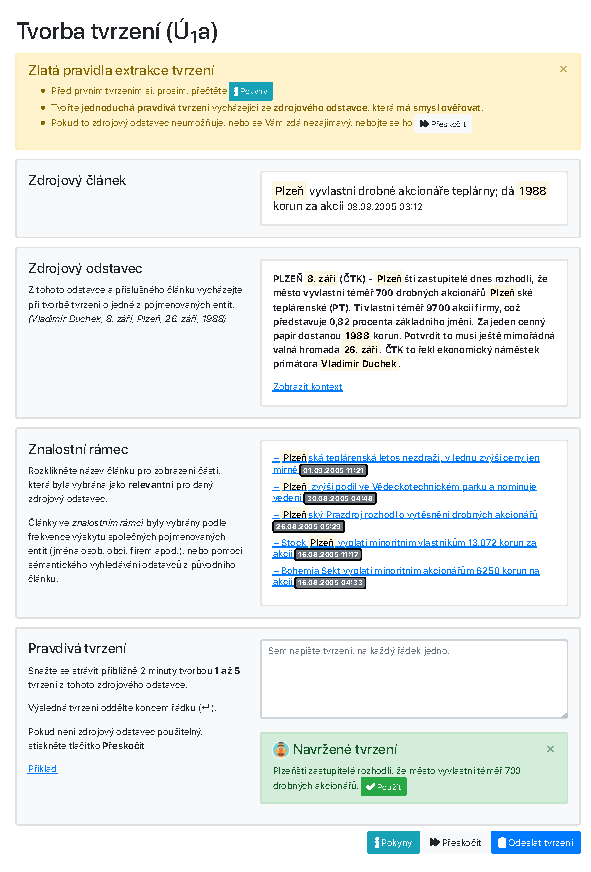
\includegraphics[height=7.5cm]{fig/fcheck/claim_extraction.pdf}
    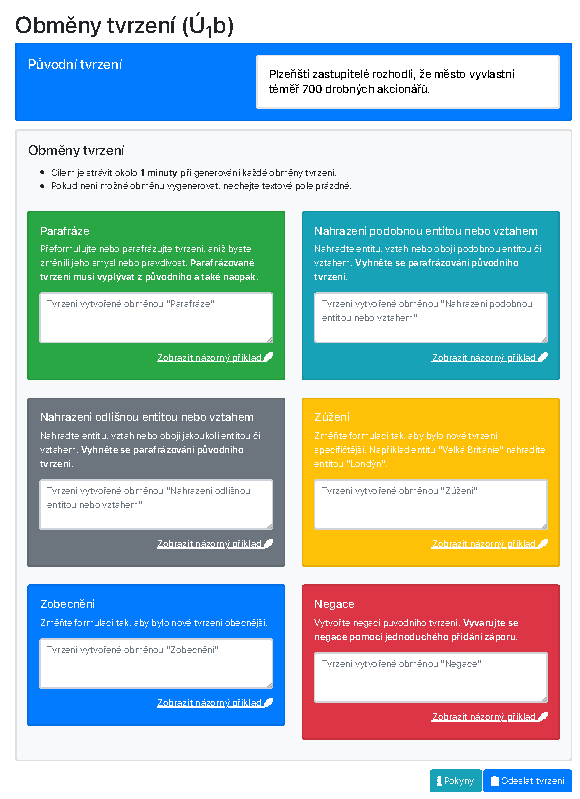
\includegraphics[height=7.5cm]{fig/fcheck/mutation.pdf}
    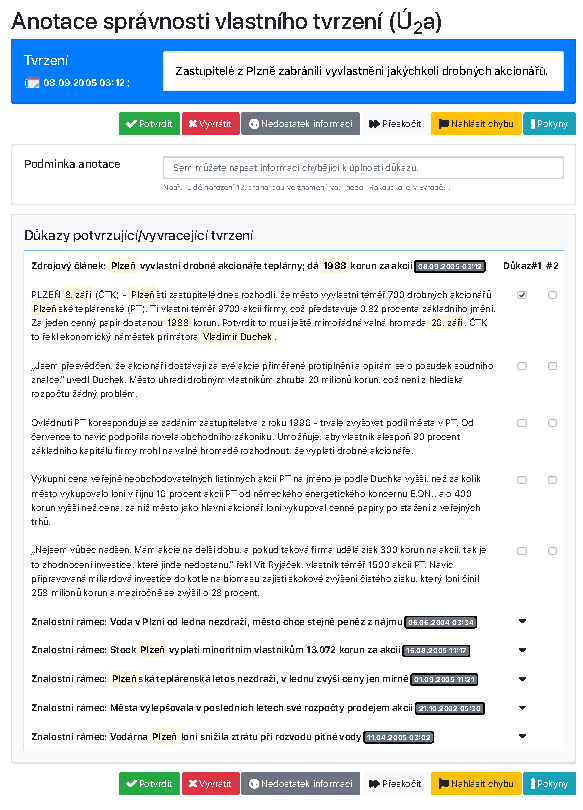
\includegraphics[height=7.5cm]{fig/fcheck/annotation.pdf}
    }
    \caption{{\techbf FCheck} -- platform for fact-checking data collection developed for TAČR project; collects data for claim generation, information retrieval and natural language inference tasks}
    \label{fig:fcheck}
\end{figure}

We have established a 4-step annotation procedure inspired by the time-proven methodology of~\cite{fever} where chech-worthy paragraphs are first hand-picked among samples from the whole archive of ČTK's 3.3 M news reports published between 1 January 2000 and 6 March 2019. Then, the annotator is sampled such a paragraph and asked to \textit{extract claims} from it, i.e., formulate single-sentence summaries of some facts that appear in paragraph. This claim is always \textit{supported} by the data, so the next phase is to perturb the claim by annotator's world knowledge and form the claim \textit{mutations} -- substitutions of entities, generalizations, specifications, paraphrases or negations of the original claim. 
The mutated claim is then fact-checked by (typically) another annotator, using the ČTK data narrowed down to a reasonable number of relevant articles (in an IR sense) as \textit{supportable}, \textit{refutable} or \textit{not enough info}, providing a set of evidence as a verdict justification.

The whole application is running on multiple levels -- a yii-framework-powered PHP app is running the annotation interface, while a flask server in python is running our models based on TF-IDF~\cite{drqa} and mBERT (section~\ref{sec:bert}) for information retrieval trained among other data on the \FCZ dataset (section~\ref{sec:fcz}).
The models are solving the Information Retrieval task on-demand (with cache) on the proprietary ČTK corpus, whenever the annotation app needs it to provide a context to the fact-checker.

The scheme and its implementations are exhaustively described in~\cite{diplomka}, chapter 4 and in~\cite{lrev}, also chapter 4.
Multiple \"{cross-annotations} were collected for each claim, to measure agreement and give insights into task complexity.

\subsection{\CTK}
\label{sec:ctkfacts}


After completing the first year of annotation experiments, we have extracted a total of 3,116 multi-annotated claims.
47\% were \texttt{SUPPORT}ed by the majority of their annotations, \REF{} and \NEI{} labels were approximately even, the full distribution of labels is listed in Table~\ref{tab:ctkfacts}.
% We have originally experimented with balanced \dev and \test splits to punish predictors exploiting this bias.

\begin{table}[H]
    \makebox[\textwidth][c]{
    \begin{ctucolortab}
    \begin{tabular}{ r || ccc || ccc  }
    &  \multicolumn{3}{c}{\techbf{{\CTK}}} uncleaned, balanced & \multicolumn{3}{c}{\techbf{{\CTK}} (launch)} cleaned, stratified\\
    \hline
    {} & {\texttt{SUPPORTS}} & \texttt{REFUTES}  & \texttt{NEI} & {\texttt{SUPPORTS}} & \texttt{REFUTES}  & \texttt{NEI}\\ 
    \hline
    \train  & 1,164 & 549 & 503     & 1,104 & 556 & 723 \\
    \dev    & 100 & 100 & 100       & 142 & 85 & 105\\
    \test   & 200 & 200 & 200       & 176 & 79 & 127\\
    \end{tabular}
    \end{ctucolortab}}
    \caption{Label distribution in \CTK splits before and after cleaning. Reprinted from~\cite{lrev}}
    \label{tab:ctkfacts}
    \end{table}

Of all the annotated claims, 1,776, that is 57\%, had at least two independent labels assigned by different annotators.
I used this multiplicity to asses the quality of our data and ambiguity of the task, as well as to propose annotation cleaning methods used to arrive to our final \text{cleaned} \CTK dataset.

\subsubsection{Inter-Annotator Agreement}
\label{sec:agreement}

Due to our cross-annotation design, I had generously sized sample of independently annotated labels in our hands.
As the total number of annotators was greater than 2, and as missing observations were allowed, I have used the Krippendorff's alpha measure~\cite{krippendorff1970} which is the standard for this case~\cite{hayes2007krippendorff}.
For the comparison with \cite{fever} and \cite{norregaard2021danfever}, I also list a 4-way Fleiss' $\kappa$-agreement~\cite{fleiss1971measuring} calculated on a sample of 7.5\% claims.

I have calculated the resulting Krippendorff's alpha agreement to be 56.42\% and Fleiss' $\kappa$ to be 63\% and interpreted this as an adequate result that testifies to the complexity of the task of news-based fact verification within a fixed knowledge scope.
It also encourages a round of annotation cleaning experiments that would exploit the number of cross-annotated claims to remove common types of noise.

\subsubsection{\CTK publication}
\CTK dataset was then subject to a thorough human-in-the-loop data cleaning until a 100\% agreement among the data was reached, in order to remove data that contains obvious noise and reveal phenomena that lead to erroneous annotations.
The full process as well as it results are described in~\cite{lrev}.

Ultimately, a dataset of 3.1K thorougly cleaned data points in a form of a factual claim, its veracity label and justifications consisting of ČTK paragraphs was published in a version for Information Retrieval\footnote{\url{https://huggingface.co/datasets/ctu-aic/ctkfacts}} for those who have access to the ČTK knowledge base to retrieve from, as well as in a special version for the task of Natural Language Inference\footnote{\url{https://huggingface.co/datasets/ctu-aic/ctkfacts_nli}} containing all the required ČTK excerpts we have negotiated to publish under open license for everyone to use.

The datasets have become our standard benchmark within the AIC NLP group~\cite{semin,mlynar} and are starting to be referred and used in others' research in the field~\cite{stefanik}.

\subsection{Other NLP datasets in West Slavic languages}
Over the time, we have accumulated numerous sets of data in Czech and other Slavic languages that have previously been poorly covered or not available at all, some of which are to be referred in our future publications.
For the convenience of others, most of them are already listed in our public repositories.
Let us mention some significant examples:

\begin{enumerate}
    \item We have machine-translated the most popular NLI training and benchmark datasets such as Stanford NLI~\cite{snli:emnlp2015}, Adversarial NLI~\cite{anli} and MultiNLI~\cite{multinli} picking a machine translator empirically for each dataset between DeepL~\cite{deepl}, Google Translate~\cite{googletranslation} and CUBBITT~\cite{popel2020Transforming}.
    
    The resulting datasets can are maintained at our public repositories:
    \begin{enumerate}
        \item \url{https://huggingface.co/datasets/ctu-aic/snli_cs}
        \item \url{https://huggingface.co/datasets/ctu-aic/anli_cs}
        \item \url{https://huggingface.co/datasets/ctu-aic/multinli_cs}
    \end{enumerate}
    \item For the task of claim generation we are establishing and performing in Czech, we have adapted the existing related datasets and are working with:
    \begin{enumerate}
        \item CTKSum -- \url{https://huggingface.co/datasets/ctu-aic/ctksum} based on source articles and extracted claims within the original \CTK{} set
        \item FEVERSum (based on FEVER Wikipedia abstract and extracted claims) -- \url{https://huggingface.co/datasets/ctu-aic/fever-sum}
        \item Its DeepL translation CsFEVERSum -- \url{https://huggingface.co/datasets/ctu-aic/csfever-sum}
        \item Our reproduction of a crawled Slovak summarization dataset described by~\cite{suppa-adamec-2020-summarization} SMESum based on articles from \url{https://sme.sk} -- \url{https://huggingface.co/datasets/ctu-aic/smesum}
    \end{enumerate}
\end{enumerate}
Up until now, some of the data was restricted to private repositories, but with this study, I am publishing most of them, as I have now found the licensing to be rather relaxed.
If some of the repositories reader might be interested in would not be reachable, please request access to the  \url{https://huggingface.co/datasets/ctu-aic} organization to be able to see into the private part of our dataset library.

\section{Models}
\label{sec:models}
The most significant pretrained models I have made public address two tasks -- the Natural Language Inference and Claim Generation viewed as a form of Abstractive Summarization task.
\subsection{Natural Language Inference}
My previous work~\cite{diplomka, lrev} also focused on establishing a strong starting state of the art on our own datasets in the tasks of NLI.
In my publications, I have tried and compared a multitude of neural networks for the tasks, ultimately arriving to:
\begin{itemize}
    \item {\techbf XLM-RoBERTA-Large@XNLI@\FCZNLI}, a model with 561M parameters trained on 100-language CommonCrawl corpus finetuned on multilingual XNLI~\cite{conneau2018xnli} inference datased and then finetuned \textit{again} on the \FCZNLI task yields an unmatched 73.7\% F1 macro score on the denoised \FCZNLI inference task: \url{https://huggingface.co/ctu-aic/xlm-roberta-large-xnli-csfever_nli}
    \item {\techbf XLM-RoBERTA-Large@SQuAD2}, a model version finetuned on a Question answering SquAD2~\cite{squad} task has shown remarkable practicality in my NLI applications and after task specific finetuning, it was able to tackle:
    \begin{enumerate}
        \item \CTKNLI\footnote{\url{https://huggingface.co/ctu-aic/xlm-roberta-large-squad2-ctkfacts_nli}} task with 76.9\% macro-F1
        \item \FCZ\footnote{\url{https://huggingface.co/ctu-aic/xlm-roberta-large-squad2-csfever_nearestp}} (noisy) task with 83.2\% macro-F1
        \item The original English FEVER NLI task\footnote{\url{https://huggingface.co/ctu-aic/xlm-roberta-large-squad2-enfever_nli}}~\cite{fever,nie2019combining}, achieving 75.9\% macro-F1 and a significant superiority over previous shared task winner~\cite{nie2019combining} (which had 69.5 macro-F1 with NSMNs)
    \end{enumerate}
\end{itemize}

\subsection{Claim generation}
In my current research, I am finding appropriate configurations and data to train models for the task of claim generation -- generating a factual claim (or more) into a single sentence that contains a fluent, atomic, decontextualized and faithful claim.
In section~\ref{generation}, I~propose the claim generation as an abstractive summarization setting, and therefore, the models already have their practical use in the general task of summing up longer texts into shorter ones.

As has been shown in section~\ref{benchmarking-sota}, NLP summarization task does not have a reliable standard benchmark that would capture all its required output qualities. Therefore, it remains questionable to claim the state of the art on any summarization task and I proceed to present models that excel in our empirical tests and demonstrations for project stakeholders:

\begin{enumerate}
    \item {\techbf mBART}~\cite{mbart} multilingual Transformer model has been finetuned by our team's~\cite{krotil} on SumeCzech and proprietary CNC News summarization dataset on the \"{full text to headline} task, obtaining encouraging scores across numerous summarization metrics in Czech.\\
    I have taken this model a step further for the claim generation task, finetuning it on the {\FCZ}Sum and {\CTK}Sum datasets, yielding a working model for the task.\footnote{
    \url{https://huggingface.co/ctu-aic/mbart25-large-eos}}

    Another experiments are being carried out with the same model finetuned on Slovak\footnote{\url{https://huggingface.co/ctu-aic/mbart-at2h-cs-smesum-2}} and Polish\footnote{\url{https://huggingface.co/ctu-aic/mbart-at2h-cs-polish-news3}} data.
    \item {\techbf LLaMA-2} shows promissing result when it comes to claim generation.
    I have finetuned\footnote{\url{https://huggingface.co/ctu-aic/Llama-2-7b-xlsum-en}} it using the QLoRA (section~\ref{sec:lora}) approach, XL-Sum~\cite{xlsum} dataset and a concatenation-based prompting strategy~\cite{llama2}, to facilitate training across the entire length of input.
    
\end{enumerate}

All prototype models are currently being iterated with our CEDMO project partners (fact-checkers from European organizations),  tweaked, and future tests are being designed for them based on empirical results and questionnaires.


\section{Applications}
\label{sec:applications}
Several applications demonstrating our contributions are currently deployed and available online due to the CEDMO project and their testing with future users, let us therefore present the main applications I and my supervisor Jan Drchal have developed for the tasks:

\begin{enumerate}
    \item Claim extractor at \url{https://fcheck.fel.cvut.cz:1830} (figure~\ref{fig:claimgencedmo}) demonstrates the single or multiple claim generation task with our LLaMA-2 or mBART models for English and Czech texts, respectively, using a GRADIO interactive application and an API
    \item  \url{https://fcheck.fel.cvut.cz:1831} runs a FactSearch platform by Jan Drchal, demonstrating our best performing models for the whole fact-checking tasks, integrating the XLM-RoBERTas trained on \FCZNLI data
    \item  \url{https://fcheck.fel.cvut.cz:1832} runs the same scheme with our best performing English models and data
\end{enumerate}

\begin{figure}
    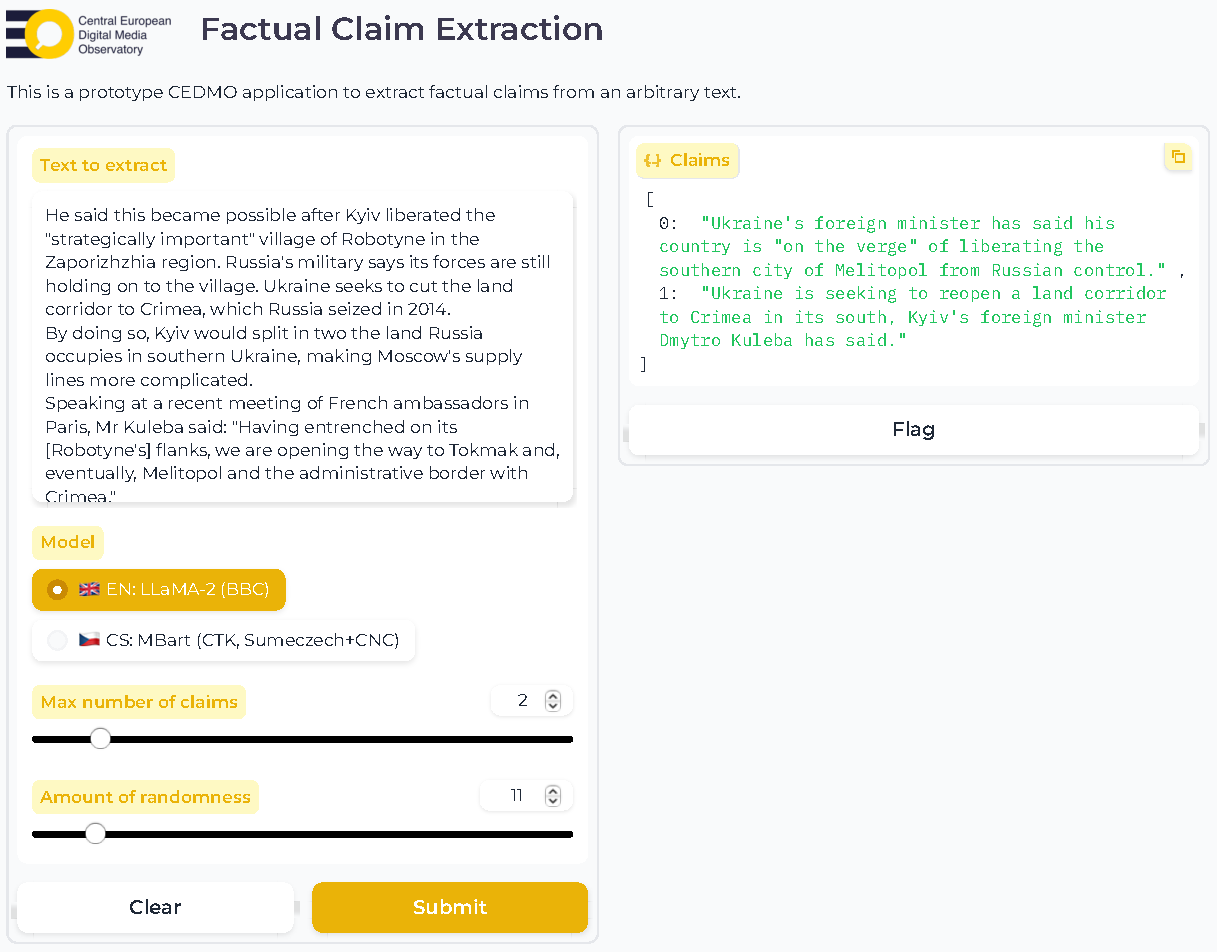
\includegraphics[width=16cm]{fig/cedmo.pdf}
    \caption{Factual claim extraction application done for the CEDMO project}
    \label{fig:claimgencedmo}
\end{figure}

Here we will show off the demonstration tools, as well as our open-source platform \url{https://fcheck.fel.cvut.cz} and currently running claim extraction tools. 
%!TEX ROOT=../ctutest.tex

\chapter{Dissertation plan}
\label{chap:plan}

%!TEX ROOT=../ctutest.tex

\chapter{Conclusion}
\label{chap:conclusion}
In this study, I have presented my current challenges and their motivation -- a desire for an automated scheme to assist fact-checking.
The solutions are being proposed in other literature and rely mostly on transformers, which is the current state of the art for nearly every NLP task.
The transformer usage paradigm is shifting (from the approach of \textit{fine-tuning} a \textit{pre-trained} transformer to \textit{prompting} or \textit{few-shotting} a Large Language Model), which will impact my dissertation and also yield new challenges in modernizing our previous work.

So far, numerous datasets, most notably the \FCZ and \CTK, have been collected, a working fact-checking pipeline was deployed on them, and the models we trained were published for further use.

Other tasks are to be established among the scientific public, importantly the claim generation and its model-based metrics, ongoing research such as the claim generation model training, collection of additional data in Czech, English, Polish, and Slovak is to be concluded, and new solutions for the whole problem of automated fact-checking are to be proposed, utilizing the new SOTA methods, such as the Large Language Models.

The point of the precedent chapters of the study was to give insights on what has been done so far, what is its value, what is the context in which this is happening, and what are the likely next steps in the future of my research.

%\bibliographystyle{amsalpha}
\bibliographystyle{apalike}
\bibliography{minimum}
\appendix
%\chapter{Czech-English data translations}
\section{Translated figures}

\begin{figure}[H]
\centering
 \fbox{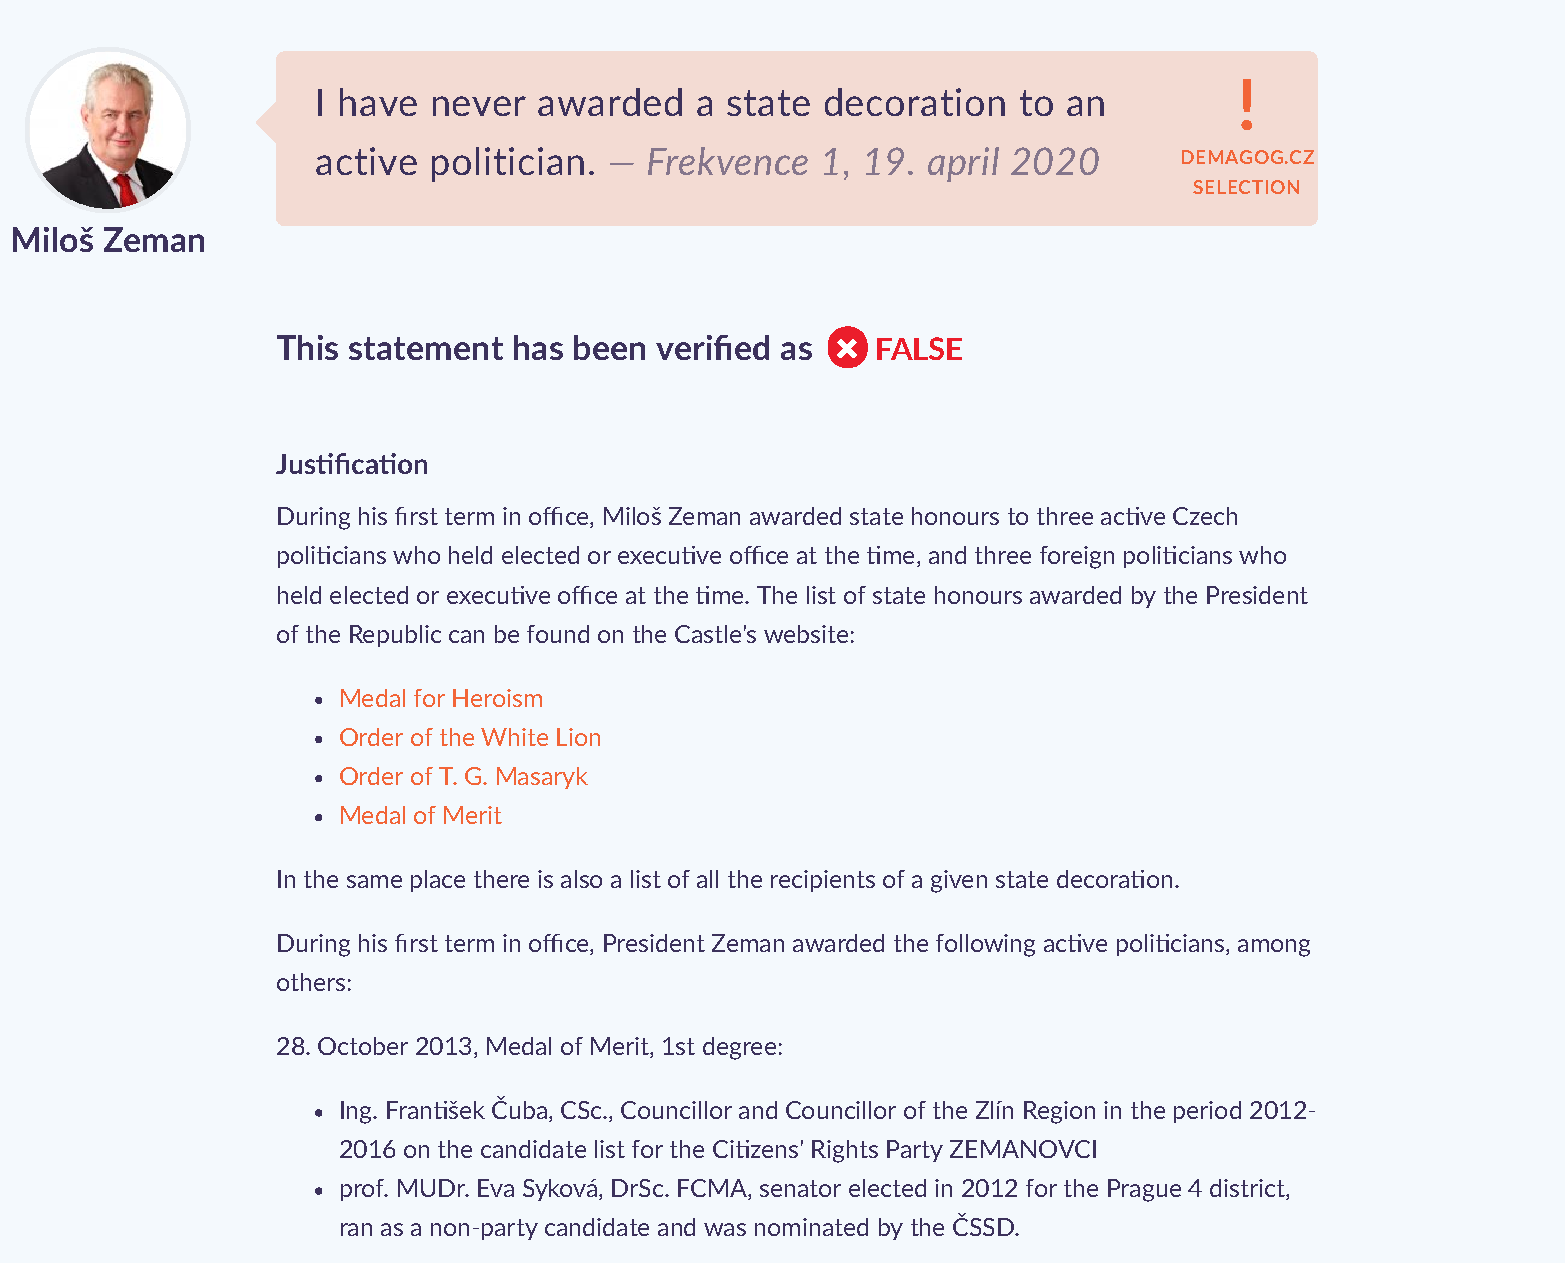
\includegraphics[width=\textwidth]{fig/demagog_en.pdf}}
\caption[English Translation of Figure~\ref{fig:demagog}]{Translated fact verification from Czech portal \textsf{Demagog.cz} -- original in Figure~\ref{fig:demagog}}
\label{trans:demagog}
\end{figure}

\begin{figure}
\thisfloatpagestyle{empty}
\vspace{-2cm}
 \makebox[\textwidth][c]{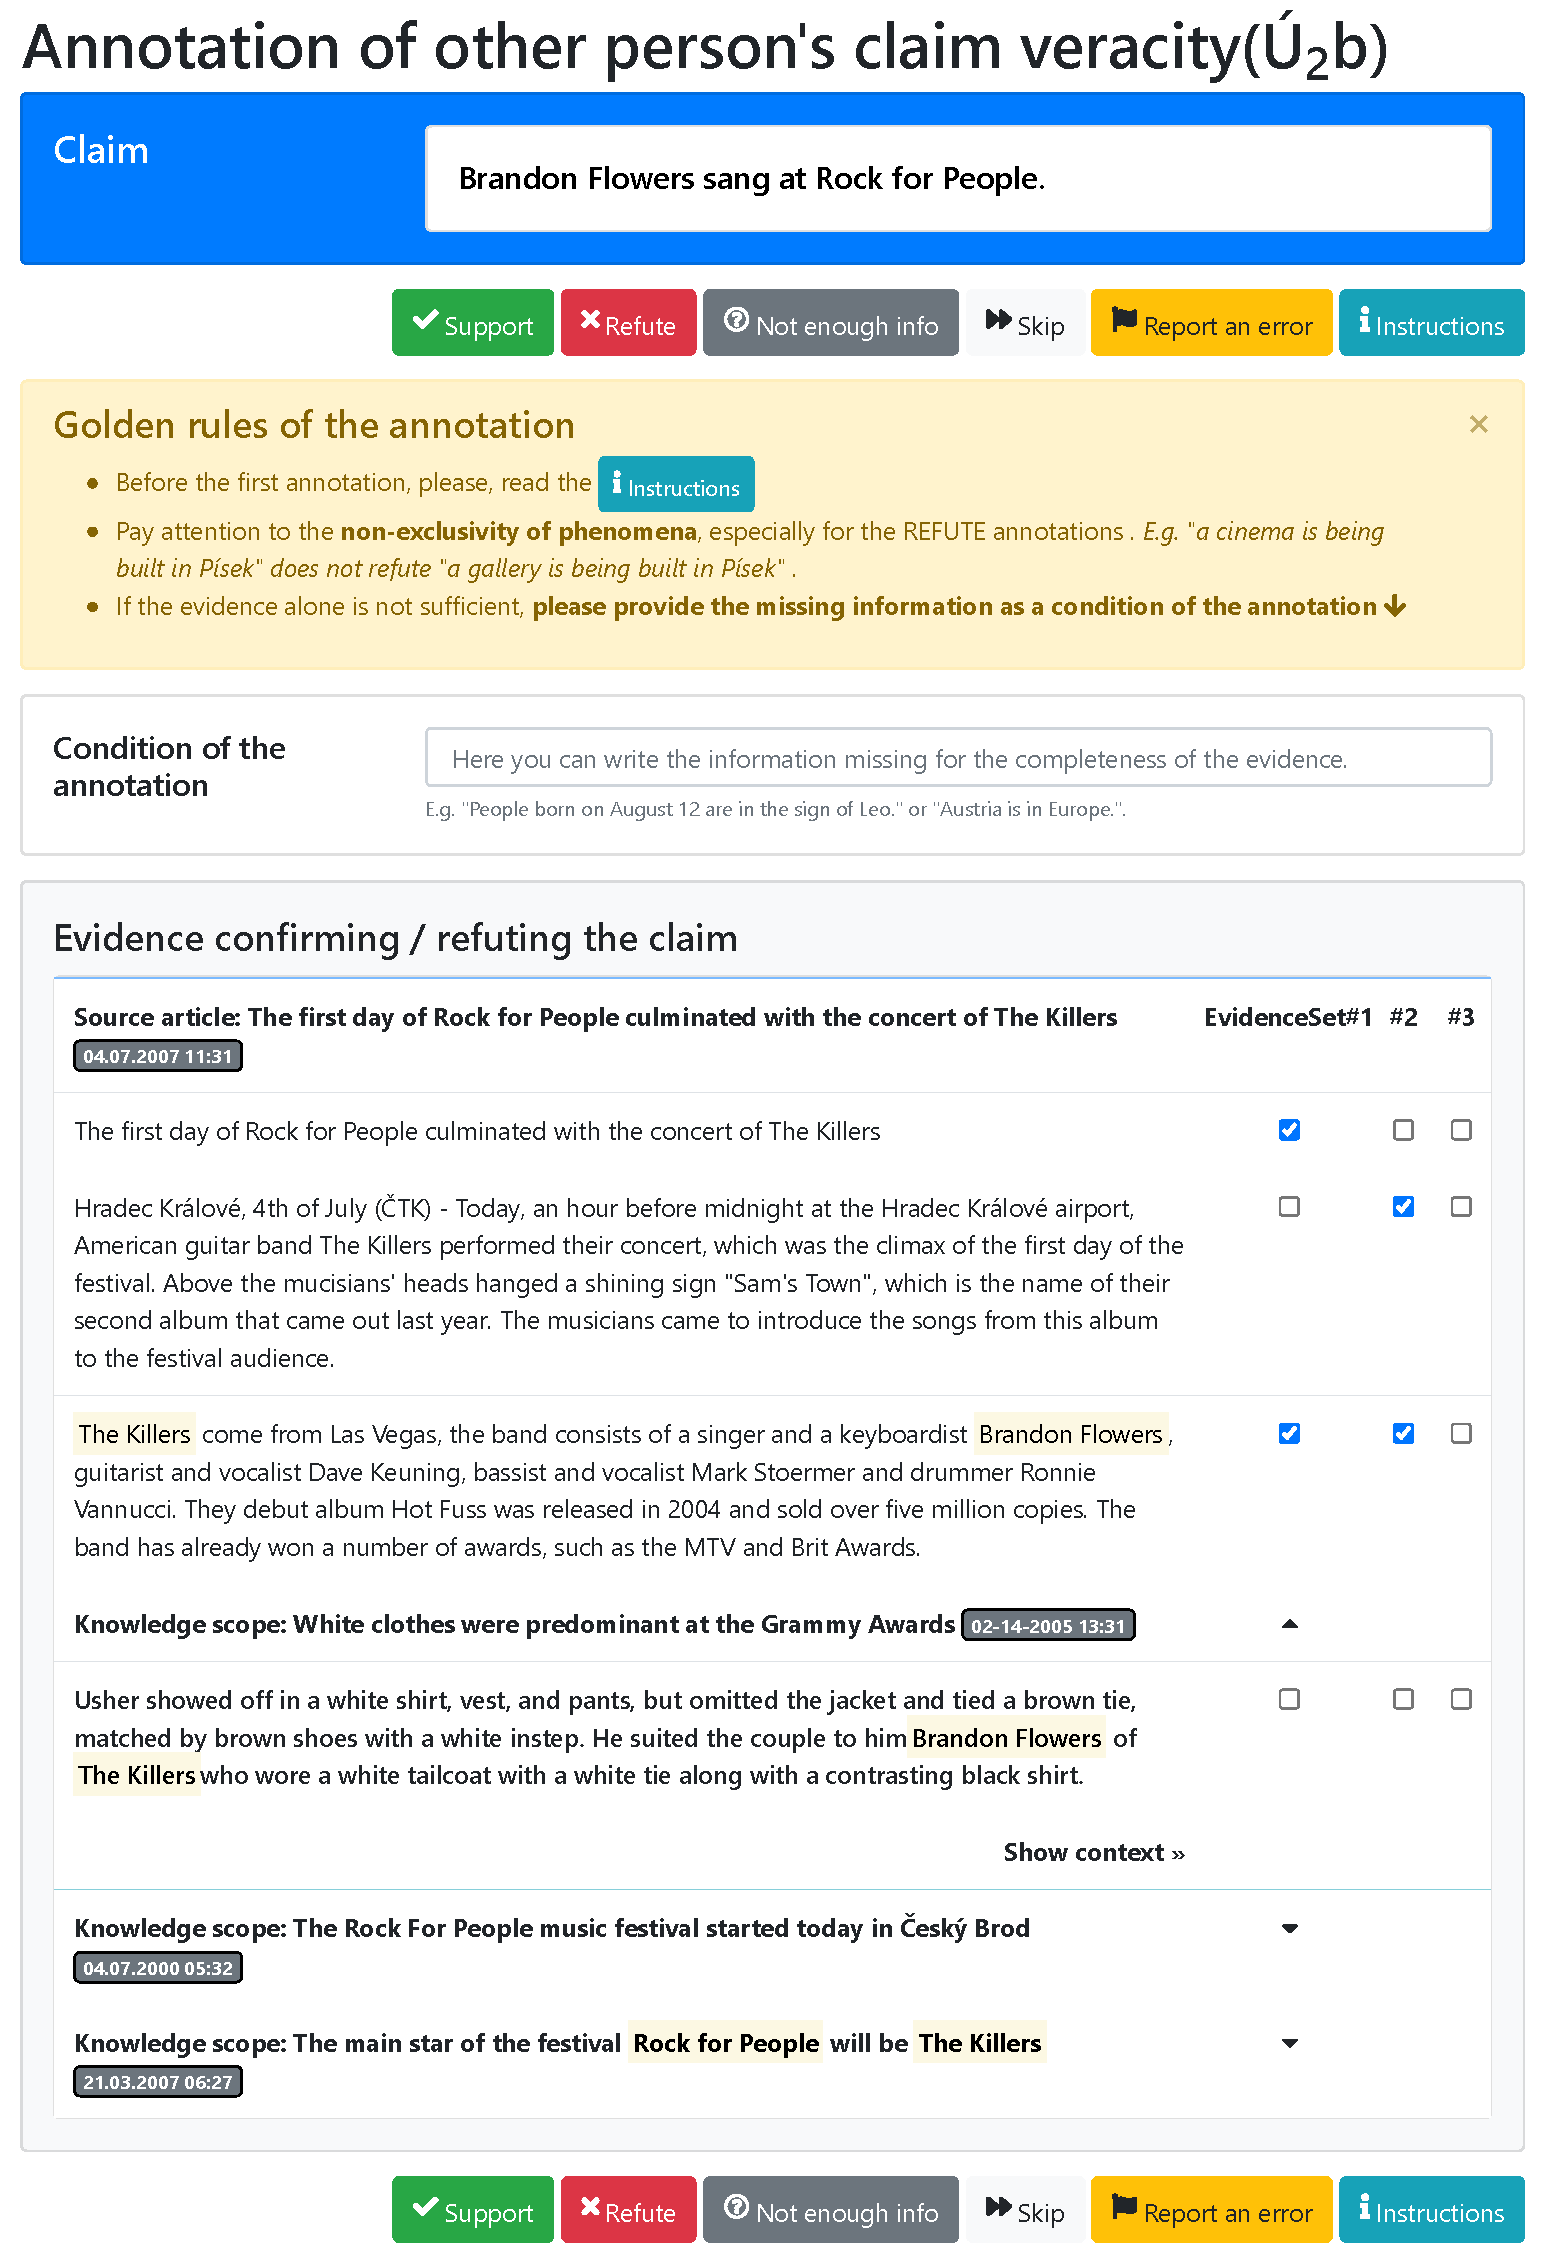
\includegraphics[width=18cm]{fig/annotation_en.pdf}}
\caption[English Translation of Figure~\ref{fig:annotation}]{The labelling interface of \textsf{FCheck} platform. Czech original in Figure~\ref{fig:annotation}}
\label{trans:annotation}
\end{figure}

\chapter{Acronyms}
\begin{description}
\item[BERT] Bidirectional Encoder Representations from Transformers
\item[GPT] Generative Pre-trained Transformer 
\item[FEVER] Fact Extraction and Verification -- series of Shared tasks focused on fact-checking
\item[CLI] Command-Line Interface
\item[NLI] Natural Language Inference
\item[ČTK] Czech Press Agency
\end{description}


\end{document}